\documentclass[xcolor=table, handout]{beamer}

\usepackage{shyne}

% Theme settings
\setbeamertemplate{navigation symbols}{}

\usetheme{Madrid}
\usefonttheme{structurebold}
\usefonttheme[onlymath]{serif}

\AtBeginSection[]
{ 	\begin{frame}{}

	{
	\usebeamerfont{frametitle}
	\begin{beamercolorbox}
		[wd={\textwidth}, center, sep=.2in, rounded=true, shadow=true]
		{frametitle}
	Chapter \thesection\\  \secname 
	\end{beamercolorbox}
	}
	
	\end{frame} 
}

\AtBeginSubsection[]
{ 	\begin{frame}{}

	{
	\usebeamerfont{frametitle}
	\begin{beamercolorbox}
		[wd={\textwidth}, center, sep=.2in, rounded=true, shadow=true]
		{frametitle}
	Section \thesection .\thesubsection\\  \subsecname 
	\end{beamercolorbox}
	}
	
	\end{frame} 
}

\title[Chapter 11]{Stat 201: Statistics I\\ Chapter 11 }
\author[M. Shyne]{}
\institute[Metro State]{
\includegraphics[width=1.75in]{../images/metro_logo}}
\date[7/14/2019]{
\\ \bigskip \bigskip 
\includegraphics[width=.4in]{../images/cc_big}}


\begin{document}
\frame{\titlepage}

% Chapter 11
\setcounter{section}{10}
\section{Goodness-of-Fit and Contingency Tables}


% Section 11.1
\subsection{Goodness-of-Fit}

\begin{frame}{Frequency distributions}
\begin{block}{}
\large
Recall, a \bt{frequency distribution} is a listing of counts, or number of occurrences, of data within a class (quantitative data) or category (categorical data). \\
\pause\medskip
A frequency table is a list of the distribution of a sample drawn from a population.\\
\pause\medskip
A test can be conducted to see if the population a sample is drawn from has an expected distribution.
\end{block}
\end{frame}

\begin{frame}{Frequency distributions, example}
\begin{exampleblock}{Example}
\large
\begin{itemize}
\item A six-sided die is ``fair" if the frequencies of each possible result of a roll (1 through 6) are equal.\\
\medskip
Given a sample of results from a number rolls of a particular die, a test could be conducted to test whether the die is ``fair".
\smallskip

\pause\item M\&Ms should have the following distribution of colors:\\
\smallskip
{\centering
\begin{tabular}{r | c c c c c c }
Color & Blue & Brown & Green & Orange & Red & Yellow\\
Percent & 24\% & 14\% & 15\% & 20\% & 13\% & 14\% 
\end{tabular}
\par} 
\bigskip
Given a sample a M\&Ms, a test could be conducted to test whether M\&Ms really do have that distribution of colors.
\end{itemize}
\end{exampleblock}
\end{frame}

\begin{frame}{Goodness-of-fit tests}
\begin{block}{}
\large
A \bt{goodness-of-fit test} is an hypothesis test which tests whether an observed frequency distribution matches, or fits, an expected distribution.
\begin{itemize}
\pause\item $H_0:$ The frequency counts agree with the expected distribution.
\pause\item $H_a:$ The frequency counts do not agree with the expected distribution.\\
\pause\item Test statistic follows a $\chi^2$ (chi-squared) distribution with $k-1$ degrees of freedom\\
\medskip
{\centering
$\ds \chi^2 = \sum \frac {(O-E)^2}{E}$
\par}
\medskip
where
\begin{itemize}
\item $k$ is the number of classes or categories
\item $O$ is the observed count for each class or category, from sample
\item $E$ is the expected count for each class or category if the expected distribution is true
\end{itemize}
\end{itemize}
\end{block}
\end{frame}

\begin{frame}{Expected counts}
\begin{block}{}
\large
The expected count for each class or category can be calculated by\\
\medskip
{\centering
$\ds E = P(c) \times n$
\par}
\medskip
where
\begin{itemize}
\item $P(c)$ is the probability of class or category $c$
\item $n$ is the sample size
\end{itemize}
\pause\medskip
For expected uniform distributions, since $P(c) = 1/k$ where $k$ is the number of classes or categories, the expected count for each class is\\
\medskip
{\centering
$\ds E  = \frac 1 k \times n = \frac n k$
\par}
\medskip
\end{block}
\end{frame}

\begin{frame}{Expected counts, example}
\begin{exampleblock}{Example}
\large
\begin{itemize}
\item Since a ``fair" die has a uniform frequency distribution, the expected counts for each result for a sample of 100 die rolls is\\
\medskip
{\centering
$\ds E = \frac n k = \frac {100} 6 = 16.67$
\par}
\medskip

\pause\item Blue M\&Ms are expected to have a frequency of 24\%. Thus, out of a sample of 150 M\&Ms, the expected count for blue is\\
\medskip
{\centering
$\ds E = P(c) \times n = 0.24 \times 150 = 36$
\par}
\medskip


\end{itemize}
\end{exampleblock}
\end{frame}

\begin{frame}{Decisions for goodness-of-fit tests}
\begin{block}{}
\large
Like most hypothesis tests, there are two ways to make a decision for a goodness-of-fit test:
\begin{itemize}
\pause\item P-value: If the calculated p-value is less than the significance level ($p < \alpha$), then reject the null hypothesis.
\pause\item Critical value: If the calculated test statistic is greater than the critical value for the significance level and degrees of freedom ($\chi^2 > \chi^2_{\alpha, k-1}$), then reject the null hypothesis. Critical values can be found in Table A-4.
\end{itemize}
\pause\medskip
For both methods, if conditions are not met to reject, fail to reject the null hypothesis.\\
\pause\medskip
Note: Chi-square test statistics are always positive and chi-square tests are always one-sided. Large values of $\chi^2$ cause rejection of the null.
\end{block}
\end{frame}

\begin{frame}{Chi-square distribution}
\bigskip
{\centering
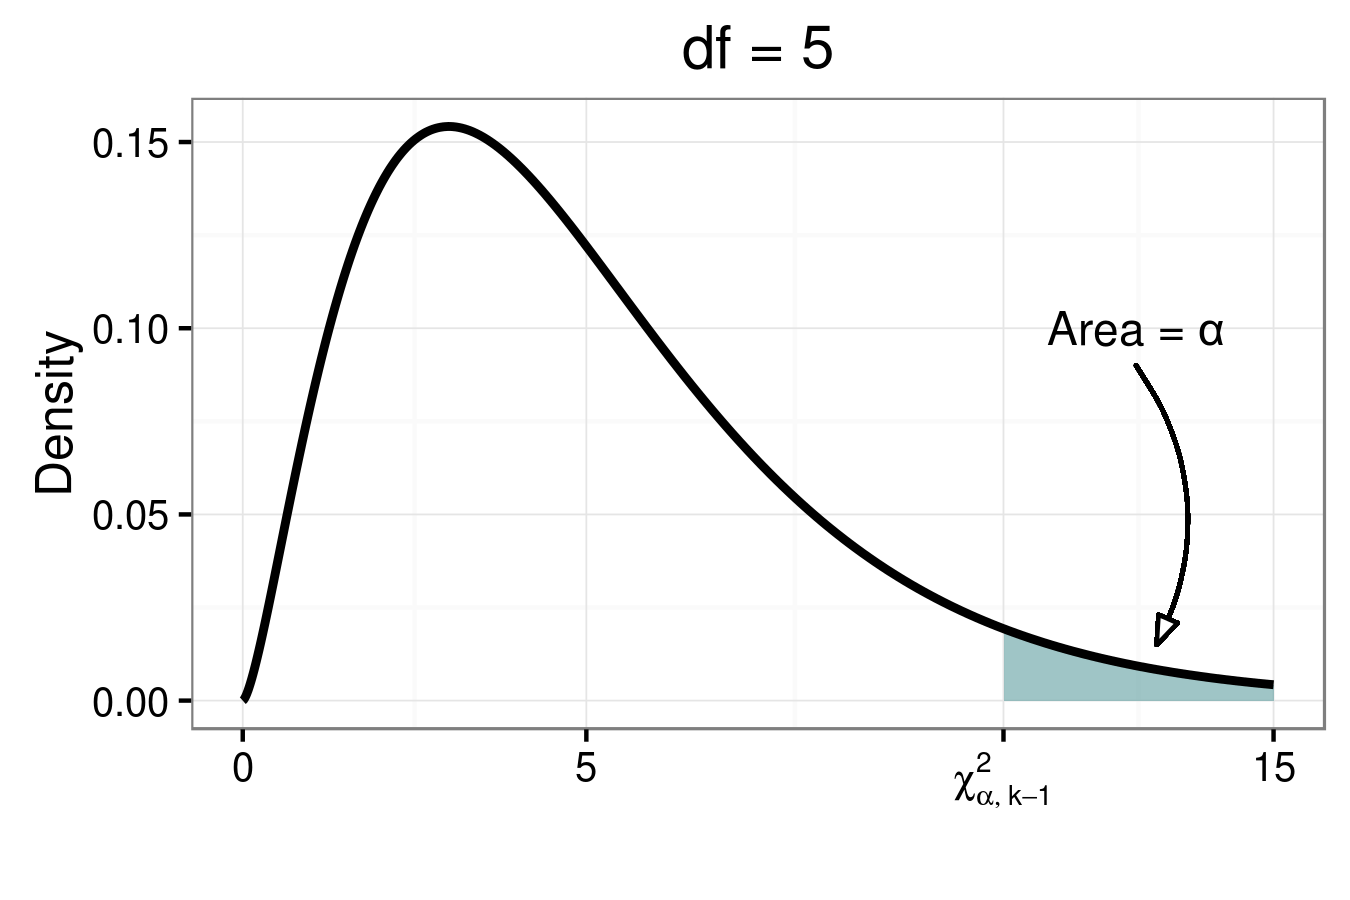
\includegraphics[width=4.5in]{../images/ch11_chi_square_crit}
\par}
\end{frame}



\begin{frame}{Requirements for goodness-of-fit tests}
\begin{block}{}
\large
\begin{itemize}
\item The sample is a simple random sample
\pause\item The sample data consists of frequency counts for each of the different categories
\pause\item For each class or category, the expected count is at least 5 
\end{itemize}
\end{block}
\end{frame}



\begin{frame}{Uniform goodness-of-fit test, example}
\begin{exampleblock}{Example}
\large
To determine if there is evidence is is not a die is ``fair", roll the die 40 times and perform a goodness-of-fit test on the results. \\
\medskip
A ``fair" die will have a uniform frequency distribution, so each result has a probability of 1/6 (16.67\%).
\medskip
\begin{itemize}
\pause\item $H_0:$ The frequency distribution of rolls fits a uniform distribution\\
$H_a:$ The frequency count of at least one result differs from the others

\pause\item Requirements: The expected count for each result is $E = \frac 1 6 \times 40 = 6.667 > 5$
\pause\item Find test statistic $\chi^2$, p-value and report decision
\end{itemize}
\end{exampleblock}
\end{frame}


\begin{frame}<handout:0>{Group work}
\begin{block}{}
\large
\begin{itemize}
\item Complete question 1.
\end{itemize}
\end{block}
\end{frame}


% Section 11.2
\subsection{Contingency Tables}

\begin{frame}{Contingency tables}
\begin{block}{}
\large
Recall, a \bt{contingency table} is a two dimensional table (rows and columns) displaying frequency counts of classes or categories of two factors for a single sample.
\end{block}
\end{frame}

\begin{frame}{Contingency tables, example}
\large
\begin{exampleblock}{Example}
Recall the cancer screening example. A sample of 1000 randomly selected people where given a new screening test for a particular kind of of cancer. Each subject either has cancer or doesn't, and either tested positive or tested negative.\\
\medskip
{\centering
\begin{tabular}{c | c  c}
\multicolumn{1}{c}{} & \multicolumn{2}{c}{Test Result}\\
Diagnosis & Positive & Negative\\
\hline
Cancer & 74 & 13\\
No cancer & 26 & 887 \\
\end{tabular}
\par}
\smallskip

\end{exampleblock}
\end{frame}

\begin{frame}{Contingency tables, example}
\begin{exampleblock}{Example}
\large
Recall the example of the school distract attempting to reduce the rate of teen drivers who text or email. The school distract created an educational program that was attend by about half the students. Afterwards, a survey was taken of a sample of teen drivers. Each teen driver either attended the program or didn't, and either texted or emailed while driving or didn't.\\
\medskip
{\centering
\begin{tabular}{c | c  c}
\multicolumn{1}{c}{} & \multicolumn{2}{c}{Texted or emailed?}\\
Attended program? & Yes & No\\
\hline
Yes & 62 & 150\\
No & 59 & 114 \\
\end{tabular}
\par}
\smallskip

\end{exampleblock}
\end{frame}


\begin{frame}{Independence in contingency tables}
\begin{block}{}
\large
An important question that can be asked about data in contingency tables is whether the two factors are independent.\\
\pause\medskip
Factors are independent if the value of one factor does not impact the value of the other factor. In other words, if the probability of being in a category of one factor does not change depending on the category of the second factor, for all categories of both factors, then the factors are independent 
\end{block}
\end{frame}

\begin{frame}{Independence in contingency tables}
\begin{exampleblock}{Example}
\large
\begin{itemize}
\item For the cancer screening example, if the probability of testing positive is the same regardless of whether the subject has cancer or not, then the test results and cancer status are independent.

\pause\item For the teen driver example, if the probability of a teen driver texting or emailing is the same regardless of whether they attended the educational program or not, then texting or emailing and program attendance are independent.
\end{itemize}
\end{exampleblock}
\end{frame}

\begin{frame}{Test for independence}
\begin{block}{}
\large
A \bt{test for independence} is an hypothesis test which tests whether data contained in a contingency table represents two factors that are independent.
\begin{itemize}
\pause\item $H_0:$ The two factors are independent
\pause\item $H_a:$ The two factors are dependent\\
\pause\item Test statistic follows a $\chi^2$ (chi-squared) distribution with $(r-1) \times (c-1)$ degrees of freedom\\
\medskip
{\centering
$\ds \chi^2 = \sum \frac {(O-E)^2}{E}$
\par}
\medskip
where
\begin{itemize}
\item $r$ is the number of rows and $c$ is the number of columns
\item $O$ is the observed count for each table cell, from sample
\item $E$ is the expected count for each table cell if the factors are independent
\end{itemize}
\end{itemize}
\end{block}
\end{frame}

\begin{frame}{Expected counts}
\begin{block}{}
\large
Like with goodness-of-fit tests, the expected count for each cell is the probability for that cell under the null hypothesis times the sample size.\\
\medskip
{\centering
$\ds E = P(c) \times n$
\par}
\pause\medskip
Recall, if events are independent that the probability of both being true is the product of the probabilities of both.\\
\medskip
{\centering
$\ds P(A \text{ and } B) = P(A) \times P(B)$
\par}
\pause\medskip
Thus, if $A$ is an event of one factor and $B$ is an event of the other factor, the expected count for the cell of $A$ and $B$ is\\
\medskip
{\centering
$\ds E = P(A) \times P(B) \times n$
\par}
\medskip
\end{block}
\end{frame}

\begin{frame}{Expected counts, cont.}
\begin{block}{}
\large
The probability of an event of one factor is the marginal probability, the total count for the row or column divided by the total sample size.\\
\medskip
{\centering
\begin{tabular}{c | c  c | c}
\multicolumn{1}{c}{} & \multicolumn{2}{c}{Factor 2}\\
Factor 1 & B & $\sim$B & Total\\
\hline
A & \# (A and B) & \# (A and $\sim$B) & \# A\\
$\sim$A & \# ($\sim$A and B) & \# ($\sim$A and $\sim$B) & \# $\sim$A \\
\hline
Total & \# B & \# $\sim$B & n
\end{tabular}\\
\bigskip
$\ds P(A) = \frac {\# A}{n} \qquad P(B) = \frac {\# B} n$
\par}
\smallskip
\end{block}
\end{frame}

\begin{frame}{Expected counts, cont.}
\begin{block}{}
\large
Thus, the expected count for the cell of A and B is\\
\medskip
{\centering
$\ds E_{A,B} = P(A) \times P(B) \times n = \frac {\# A} n \times \frac {\# B} n \times n$
\par}
\pause\bigskip
After some algebra, a simpler formula for expected count is\\
\medskip
{\centering
$\ds E_{A,B}  = \frac{\# A \times \# B}{n}$
\par}
\medskip
\end{block}
\end{frame}

\begin{frame}{Expected counts, example}
\begin{exampleblock}{Example}
\large
\smallskip
{\centering
\begin{tabular}{c | c  c | c}
\multicolumn{1}{c}{} & \multicolumn{2}{c}{Test Result}\\
Diagnosis & Positive & Negative & Total\\
\hline
Cancer & 74 & 13 & 87\\
No cancer & 26 & 887 & 913 \\
\hline
Total & 100 & 900 & 1000
\end{tabular}
\par}
\bigskip
\begin{itemize}
\pause\item $\ds E_{+,\text{cancer}} = \frac {100 \times 87}{1000} = 8.7$
\pause\item $\ds E_{-,\text{cancer}} = \frac {900 \times 87}{1000} = 78.3$
\end{itemize}
\smallskip
\end{exampleblock}
\end{frame}

\begin{frame}{Expected counts, example}
\begin{exampleblock}{Example}
\large
\smallskip
{\centering
\begin{tabular}{c | c  c | c}
\multicolumn{1}{c}{} & \multicolumn{2}{c}{Test Result}\\
Diagnosis & Positive & Negative & Total\\
\hline
Cancer & 74 & 13 & 87\\
& (8.7) & (78.3)\\
No cancer & 26 & 887 & 913 \\
& (91.3) & (821.7)\\
\hline
Total & 100 & 900 & 1000
\end{tabular}
\par}
\smallskip
\end{exampleblock}
\end{frame}

\begin{frame}{Decisions for tests for independence}
\begin{block}{}
\large
Once a test statistic $\chi^2$ is found, the decision process for a test for independence is identical to the process for a goodness-of-fit test:
\begin{itemize}
\pause\item P-value: If the calculated p-value is less than the significance level ($p < \alpha$), then reject the null hypothesis.
\pause\item Critical value: If the calculated test statistic is greater than the critical value for the significance level and degrees of freedom ($\chi^2 > \chi^2_{\alpha, (r-1)(c-1)}$), then reject the null hypothesis. Critical values can be found in Table A-4.
\end{itemize}
\pause\medskip
For both methods, if conditions are not met to reject, fail to reject the null hypothesis.\\
\end{block}
\end{frame}


\begin{frame}{Requirements for tests for independence}
\begin{block}{}
\large
\begin{itemize}
\item The sample is a simple random sample
\pause\item The sample data consists of frequency counts for every cell of a contingency table
\pause\item For every cell, the expected count is at least 5 
\end{itemize}
\end{block}
\end{frame}


\begin{frame}{Test for independence, example}
\begin{exampleblock}{Example}
\large
Recall the cancer screening data:\\
\smallskip
{\centering
\begin{tabular}{c | c  c | c}
\multicolumn{1}{c}{} & \multicolumn{2}{c}{Test Result}\\
Diagnosis & Positive & Negative & Total\\
\hline
Cancer & 74 & 13 & 87\\
& (8.7) & (78.3)\\
No cancer & 26 & 887 & 913 \\
& (91.3) & (821.7)\\
\hline
Total & 100 & 900 & 1000
\end{tabular}
\par}
\bigskip
Test whether cancer diagnosis has an effect on the screening test result at $\alpha = 0.01$ level of significance.
\end{exampleblock}
\end{frame}

\begin{frame}{Test for independence, example}
\begin{exampleblock}{Example}
\large
\begin{itemize}
\pause\item $H_0:$ Test result and cancer diagnosis are independent\\
$H_a:$ Test result and cancer diagnosis are dependent (test result is associated with cancer diagnosis)
\pause\item Requirements: The smallest expected count, for cancer and positive test, is 8.7 which is larger than 5
\pause\item $\chi^2 = 596.47717$\\
$p < 0.0001 $
\pause\item $p < 0.0001 < 0.01 = \alpha$. Reject null hypothesis.
\pause\item There is evidence that test results and cancer diagnosis are associated.
\end{itemize}
\end{exampleblock}
\end{frame}

\begin{frame}{Test for independence, example}
\begin{exampleblock}{Example}
\large
Recall the teen driver data:\\
\medskip
{\centering
\begin{tabular}{c | c  c}
\multicolumn{1}{c}{} & \multicolumn{2}{c}{Texted or emailed?}\\
Attended program? & Yes & No\\
\hline
Yes & 62 & 150\\
No & 59 & 114 \\
\end{tabular}
\par}
\bigskip
Test whether texting or emailing while driving is associated with program attendance at $\alpha = 0.05$ level of significance.
\end{exampleblock}
\end{frame}

\begin{frame}{Test for independence, example}
\begin{exampleblock}{Example}
\large
\begin{itemize}
\pause\item $H_0:$ Texting or emailing and program attendance are independent\\
$H_a:$ Texting or emailing and program attendance are dependent (texting or emailing is associated with program attendance)
\pause\item Requirements: We don't have expected counts yet, but the sample size is in the hundreds and no outcome appears very unlikely. We can confirm when we have expected counts.
\pause\item $\chi^2 = 1.0435298$\\
$p = 0.307 $
\pause\item $p = 0.307 > 0.05 = \alpha$. Fail to reject null hypothesis.
\pause\item There is no evidence that texting or emailing while driving and program attendence are associated.
\end{itemize}
\end{exampleblock}
\end{frame}

\begin{frame}{Test for independence vs. proportion test}
\begin{block}{}
\large
Recall, we performed a test with this data in Chapter 9. Testing the alternative hypothesis that the proportion of teen drivers who texted or emailed while driving was lower than for teens who attended the educational program than those who did not. \\
\begin{itemize}
\pause\item The results were $z = -1.0215331, \, p = 0.307$.\\
\pause\item The test for independence, while conducted as a one-sided test, is actually a two-sided test in that is does not distinguish between observed values that are lower or higher than expected values.\\
\pause\item Thus, the test for independence gave us identical results as the equivalent proportion test.
\end{itemize}
\end{block}
\end{frame}


\begin{frame}<handout:0>{Group work}
\begin{block}{}
\large
\begin{itemize}
\item Complete questions 2 and 3.
\end{itemize}
\end{block}
\end{frame}

\end{document}